\usepackage[utf8]{inputenc}
\bibliographystyle{apalike}
\usepackage{bibentry}
\nobibliography*
\usepackage{slovak}
\usepackage{tikz}
\usetikzlibrary{arrows,positioning}
\usetheme{Warsaw}
\title{Biologicky motivované \\výpočtové modely}
\author[Mgr. Michal Kováč]{Mgr. Michal Kováč\\{\small Školiteľ: doc. RNDr. Damas Gruska, PhD.}}
\institute{FMFI UK}
\date{17.1.2018}
\begin{document}
% \renewcommand{\pause}{}

\begin{frame}[t]
\titlepage
\end{frame}
\note{
  Vážení prítomní, volám sa Michal Kováč a chcel by som vám prezentovať výsledky mojej dizertačnej práce s názvom Biologicky motivované výpočtové modely.
}

\begin{frame}
\tableofcontents
\end{frame}
\note{
  V úvode prezentácie vám predstavím rôzne výpočtové modely motivované biologiou. Najviac sme sa venovali P systémom, preto budem pokračovať formálnou definíciou a prehľadom rôznych variantov P systémov.

  V druhej časti predstavím 4 témy nášho výskumu, z čoho 3 články boli publikované. V našej práci sme skúmali viaceré varianty P systémov a to konkrétne Sekvenčné P systémy s inhibítormi, Sekvenčné P systémy s aktívnymi membránami, Sekvenčné P systémy s množinami namiesto multimnožín, z čoho všetky spomenuté témy boli publikované. Dalším variantom P systémov, ktorým sme sa zaoberali bola Detekcia prázdnosti membrán.
}

\section{Prehľad problematiky} % (fold)
\label{sec:prehlad_problematiky}

\subsection{Prehľad modelov} % (fold)
\label{sub:prehlad_modelov}

\begin{frame}[t]\frametitle{Biologicky motivované \\výpočtové modely}
  Dvojaké uplatnenie:
  \begin{itemize}
    \item reálne modely živých systémov
    \begin{itemize}
      \item virtuálne biologické experimenty
      \item verifikácia správnosti chápania ich činností
    \end{itemize}
    \item modely na popis iných systémov
  \end{itemize}
\end{frame}
\note{
  Biologicky motivované výpočtové modely majú dvojaké uplatnenie.

  Jednak v rámci biológie môžu slúžiť ako reálne modely správania sa živých systémov, na ktorých môžeme robiť rôzne virtuálne biologické experimenty, prípadne verifikovať správnosť nášho chápania ich biologickej činnosti.

  Na druhej strane môžu slúžiť ako modely na popis aj iných ako biologických systémov, čo otvára rad teoretických informatických otázok, napr. výpočtová sila alebo analýza behaviorálnych vlastností.
}

\begin{frame}[t]\frametitle{Biologicky motivované \\výpočtové modely}
  \begin{itemize}
    \item Neurónové siete (od 1943)
    \item Celulárne automaty (od 1968)
    \item Evolučné algoritmy (od 1954)
    \item L systémy (od 1968)
    \item Swarm Intelligence (od 1989)
    \item P systémy (od 1998) \cite{Paun98}
    \item \dots
  \end{itemize}
\end{frame}
\note{
  Dlho skúmané modely ako neurónové siete, celulárne automaty, evolučné algoritmy, L systémy, či swarm intelligence, si už našli svoje uplatnenie v praxi, kým membránové systémy sú ešte len v začiatkoch svojho vývoja.
}

% subsection prehlad_modelov (end)

\subsection{P systémy} % (fold)
\label{sub:p_systemy}

\begin{frame}[t]\frametitle{Membránová štruktúra}
  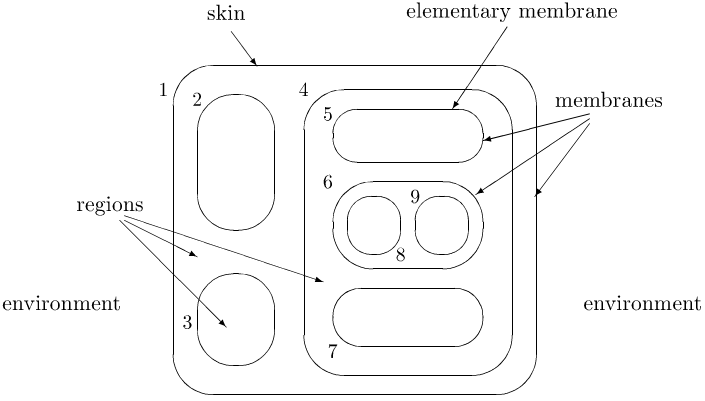
\includegraphics[width=0.7\textwidth]{membrane_structure.png}
  \hfill
  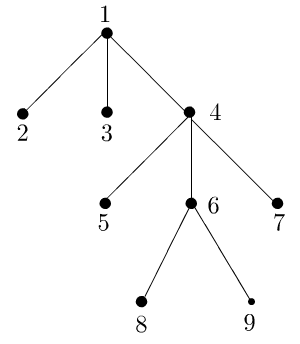
\includegraphics[width=0.3\textwidth]{membrane_tree.png}
  \pause
  \begin{itemize}
    \item Multimnožiny
    \pause
    \item Pravidlá
  \end{itemize}

\end{frame}
\note{
  Membránové systémy sú inšpirované bunkami. Základom je preto membránová štruktúra, ktorá pozostáva z regiónov, ktoré sú oddelené membránami. Tvorí to hierarchickú štruktúru, ktorá sa dá zobraziť aj ako strom.

  NEXT SLIDE

  Obsahom regionov je multimnožina objektov, ktoré v realite predstavujú napr. molekuly, vírusy, enzýmy alebo proteíny.

  NEXT SLIDE

  Objekty medzi sebou môžu interagovať. Táto interakcia je definovaná prepisovacími pravidlami.
}

\begin{frame}[t]\frametitle{Prepisovacie pravidlá}
  $u\rightarrow v$, where
  \begin{itemize}
    \item $u\in\mathbb{N}^\Sigma$
    \pause
    \item $v=v^\prime$ or $v=v^\prime\delta$, where $\delta\notin\Sigma$
    \item $v^\prime\in\mathbb{N}^{\Sigma\times(\{here, out\}\cup\{in_j|1\leq j\leq m\})}$
  \end{itemize}
\end{frame}
\note{
  Prepisovacie pravidlá majú ľavú a pravú stranu. Na ľavej strane sú reaktanty, čo je multimnožina objektov.

  NEXT SLIDE

  Na pravej strane sú produkty, čo je multimnožina objektov, pričom pre každý objekt sa definuje, či ostáva v aktuálnom regione, alebo ide cez membránu do vonkajšieho regionu alebo cez membránu s daný označením do vnútorného regionu.

  Delta je špeciálny symbol, ktorý nepatrí abecede, ktorý ked je prítomný, tak po aplikovaní pravidla sa rozpustí membrána, v ktorej sa pravidlo aplikovalo a obsah membrány sa vyleje von.

  Pravidlo je aplikovateľné v danom regione, ak sú reaktanty obsiahnuté v multimnožine objektov, ktorá sa aktuálne nachádza v danom regione.  
}

\begin{frame}[t]\frametitle{Varianty pravidiel}
  $u\rightarrow v$
  \begin{itemize}
    \item Kooperatívne ($u\in\mathbb{N}^\Sigma$) (PsRE \cite{Paun98})
    \pause
    \item Nekooperatívne ($u\in\Sigma$) (PsCF \cite{Sburlan05dragos})
    \pause
    \item Nekooperatívne s inhibítormi ($u \rightarrow v\ |_{\neg{Inh}}, Inh\subseteq\Sigma$) (PsET0L \cite{Ionescu:jucs_10_5:on_p_systems_with})
    \pause
    \item Katalytické ($cu \rightarrow cv, u\in\Sigma, c\in C\subseteq\Sigma$)
    \begin{itemize}
      \item s 2 katalyzátormi (PsRE \cite{Freund2005TwoCatalysts})
      \item s 1 katalyzátorom (otvorený problém)
      \item s 1 katalyzátorom a inhibítormi (PsRE \cite{Ionescu:jucs_10_5:on_p_systems_with})
    \end{itemize}
  \end{itemize}
\end{frame}
\note{
  Literatúra spomína rôzne spôsoby definovania prepisovacieho pravidla. Pôvodná definícia, ktorú uvádza Paun, používa kooperatívne pravidlá v znení, ako som uviedol. Takto definované P systémy sú Turingovsky úplné.

  NEXT SLIDE

  Nekooperatívne pravidlá neumožňujú interakciu medzi objektami, takže na ľavej strane je vždy iba jeden objekt. Takto definované P systémy sú ekvivalentné Parikhovmu zobrazeniu bezkontextových jazykov.

  NEXT SLIDE

  Pravidlá s inhibítormi umožňujú špecifikovať množinu objektov, inhibítorov, z ktorých ak aspoň jeden je prítomný v regione, tak dané pravidlo sa nemôže uplatniť. Takto definované P systémy sú ekvivalentné Parikhovmu zobrazeniu triedy jazykov ET0L.
}
\newpage
\note{
  Katalytické pravidlá umožňujú objektom interagovať iba s objektom z množiny katalizátorov.
  Dva katalyzátory stačia na Turingovskú úplnosť. Výpočtovú silu P systémov s jedným katalyzátorom nevieme zaradiť, je to otvorený problém. Ak ale umožníme pravidlá s inhibítormi, dosiahneme Turingovskú úplnosť.
}
    
\begin{frame}[t]\frametitle{Výpočet a jazyk}
  \begin{itemize}
    \item Krok výpočtu
    \begin{itemize}
      \item Sekvenčný
      \item Paralelný
      \item Maximálne paralelný
    \end{itemize}
    \pause
    \item Jazyk
    \begin{itemize}
      \item Generatívny mód: postupnosť objektov vypustených do okolitého prostredia
      \pause
      \item Akceptačný mód: vstupnú multimnožinu vložíme do špecifickej membrány, ak výpočet zastaví, akceptujeme
    \end{itemize}
  \end{itemize}
\end{frame}
\note{
  Postupné uplatňovanie pravidiel definuje výpočet.

  V jednom kroku výpočtu sa uplatní:
  \begin{itemize}
    \itemsep0em
    \item presne jedno pravidlo (sekv. mod)
    \item aspoň jedno pravidlo (paralelný mod)
    \item maximálna multimnožina pravidiel
  \end{itemize}

  V pôvodnej definícii, ktorú uvádza Paun, sa používa maximálny paralelizmus.
}
\newpage
\note{
  P systém definuje jazyk rôznymi spôsobmi. Môže to byť jazyk nad slovami - postupnosťami objektov alebo jazyk nad multimnožinami.
  
  V generatívnom mode môžeme zobrať objekty vypustené do prostredia počas výpočtu a túto postupnosť objektov alebo multimnožinu objektov zahrnúť do jazyka.
  Kedže pre daný P systém vdaka nedeterminizmu existuje viac možných výpočtov, veľkosť definovaného jazyka môže byť aj väčsia ako 1.
}
\newpage
\note{
  V akceptačnom mode vstupnú multimnožinu vložíme do špecifickej membrány a spustíme výpočet, ktorý ak zastaví, tak vstupnú multimnožinu zahrnieme do jazyka.

  Pre väčšinu známych modelov sú generatívny aj akceptačný mod rovnako silné, u P systémoch to nie je vždy tak, preto sa oplatí skúmať obidva mody.
}

\begin{frame}[t]\frametitle{Sekvenčné P systémy}
  \begin{itemize}
    \item Maximálny paralelizmus vs. sekvenčný mód
    \pause
    \item Sekvenčné P systémy s kooperatívnymi pravidlami (VASS \cite{Dang:2005:Sequential})
    \pause
    \begin{itemize}
      \item s prioritami (PsRE \cite{Dang:2005:Sequential})
      \item s aktívnymi membránami (PsRE \cite{Dang:2005:Sequential})
      \item {\bf s inhibítormi (PsRE \cite{Kovac14})}
    \end{itemize}    
  \end{itemize}
\end{frame}
\note{
  Maximálny paralelizmus je veľmi silná vlastnosť. Globálny časovač reakcií vo väčšine prípadov tvorí hranicu toho, čo je, a čo nie je Turingovsky úplné. Ani v bunke sa nenachádza taký časovač, podľa ktorého by sa reakcie synchronizovali. Preto sa hľadajú spôsoby, ako túto vlastnosť odľahčiť, prípadne, akými spôsobmi by sa dal rozšíriť sekvenčný mod, aby sa dosiahla Turingovská úplnosť.

  NEXT SLIDE

  Sekvenčné P systémy s kooperatívnymi pravidlami nie sú Turingovsky úplné, lebo sú ekvivalentné s Vector Addition Systems a s Petriho sieťami.

  NEXT SLIDE

  Ak sa pridajú pravidlá s prioritami, alebo s aktívnymi membránami, alebo s inhibítormi, takto definované P systémy sú už Turingovsky úplné.
}

% subsection p_systemy (end)

% section prehlad_problematiky (end)

\section{Skúmané varianty P systémov} % (fold)
\label{sec:sk_man_varianty_p_syst_mov}

\subsection{Sekvenčné P systémy s inhibítormi} % (fold)
\label{sub:sekven_n_p_syst_my_s_inhib_tormi}

\begin{frame}[t]\frametitle{Sekvenčné P systémy s inhibítormi}
  \begin{itemize}
    \item \bibentry{Kovac14}
  \end{itemize}
  \vfill\vspace{3cm}\hfill
\includegraphics[scale=0.05]{water.png}
\end{frame}
\note{
  Posledný zo spomenutých rozšírení sme prezentovali na konferencii Computability in Europe 2014 a náš článok je publikovaný v zborníku.
}


\begin{frame}[t]\frametitle{Prehľad simulácie pre akceptačný mód}
  \begin{itemize}
    \item Simulácia registrového stroja
    \pause
    \item Obsah registra $x$ sa reprezentuje početnosťou objektu $x$
    \item Objekt pre každú inštrukciu
    \pause
    \item SUB inštrukcia sa simuluje pomocou inhibítora
    \begin{itemize}
      \item $i: SUB(x,j,k)$
      \item $ix\rightarrow j$
      \item $i\rightarrow k|_{\neg{x}}$
    \end{itemize}
  \end{itemize}
\end{frame}
\note{
  Uviedli sme dôkaz Turingovskej úplnosti pre akceptačný aj generatívny mod. Pre akceptačný mod sme ukázali simuláciu registrového stroja. Obsah registra x sa reprezentuje početnosťou objektu x. Navyše máme objekt pre každú inštrukciu. Inhibítory sme využili na simuláciu inštrukcie SUB.
}

\begin{frame}[t]\frametitle{Prehľad simulácie pre akceptačný mód}
  \begin{itemize}
    \item Registrový stroj $M = (n, P, i, h, Lab)$
    \pause
    \item P systém $(\Sigma, \mu, w, R)$
    \begin{itemize}
      \item $\Sigma = Lab\cup a_j, 1\leq j\leq n\cup \#$
      \pause
      \item $w = i\cup a_i^{n_i}, n_i$ je počiatočná hodnota registra $i$
      \pause
      \item $\forall (e : add(j), k, l)\in P: $
      \begin{itemize}
        \item $e\rightarrow a_jk\in R$ 
        \item $e\rightarrow a_jl\in R$ 
      \end{itemize}
      \pause
      \item $\forall (e : sub(j), k, l)\in P: $
      \begin{itemize}
        \item $ea_j\rightarrow k\in R$ 
        \item $e\rightarrow l|_\neg{a_j}\in R$ 
      \end{itemize}
      \pause
      \item $ha_j\rightarrow h\#\in R$
      \item $\#\rightarrow\#\in R$
    \end{itemize}
  \end{itemize}
\end{frame}
\note{
  Formálne, majme registrový stroj M, kde n je počet registrov, P je množina inštrukcií označených značkami z množiny Lab, i je označenie počiatočnej inštrukcie, h je označenie koncovej inštrukcie.

  NEXT SLIDE

  Zostrojíme P systém s jednou membránou, v abecede budú označenia inštrukcií, symboly zodpovedajúce jednotlivým registrom a špeciálny ukončovací symbol mriežka.

  NEXT SLIDE

  V počiatočnej konfigurácii membrána obsahuje označenie počiatočnej inštrukcie registrového stroja a objekty $a_i$ podľa počiatočného stavu registrov.
}
\newpage
\note{
  Pre všetky inštrukcie ADD, ktoré zvýšia hodnotu registra $j$ o jedna a nasledujúca inštrukcia je k alebo l (rozhoduje sa nedeterministicky) budeme mať pravidlá, ktoré prepíše symbol zodpovedajúci označeniu inštrukcie na symbol $a_j$ a symbol zodpovedajúci označeniu nasledujúcej inštrukcie. 

  NEXT SLIDE

  Uvažujme inštrukciu SUB, ktorá ak má register $j$ kladnú hodnotu, tak ju zníži o jedna, a ak je register $j$ prázdny, tak ju nezníži, ale bude iná nasledujúca inštrukcia. Pre takáto inštrukciu budeme mať v P systéme dve pravidlá. Prvé pravidlo je kooperatívne, ktoré skonzumuje symbol $a_j$ a vytvorí symbol $k$ zodpovedajúci označeniu nasledujúcej inštrukcie. Druhé pravidlo je s inhibítorom a aplikovať sa môže len, ak sa v regione nenachádza symbol $a_j$.
}
\newpage
\note{
  Ked uvažujeme registrové stroje, kde musia byť všetky registre prázdne, aby sa výpočet korektne ukončil, máme pravidlá, ktoré pri dosiahnutí koncovej inštrukcie $h$, ak je niektorý register neprázdny, vytvorí sa špeciálny symbol, ktorý tam už ostane navždy, a vdaka poslednému pravidlu sa dosiahne, že výpočet nezastaví.

  Dokázali sme, že pre každý registrový stroj vieme zostrojiť sekvenčný P systém s inhibítormi, ktorý v akceptačnom mode zastaví na rovnakých vstupoch ako registrový stroj.
}

\begin{frame}[t]\frametitle{Prehľad simulácie pre generatívny mód}
  \begin{itemize}
    \item Simulácia maximálne paralelného P systému $\Pi_1$ pomocou sekvenčného P systému s inhibítormi $\Pi_2$.
    \pause
    \item Každý maximálne paralelný krok $\Pi_1$ simulujeme sekvenčnými krokmi $\Pi_2$.
    \pause
    \item Maximálne paralelný krok rozdeľujeme na 4 fázy:
    \pause
    \begin{itemize}
      \item RUN
      \pause
      \item SYNCHRONIZE
      \pause
      \item SENDDOWN
      \item RESTORE
    \end{itemize}
  \end{itemize}
\end{frame}
\note{
  V generatívnom mode sme sa rozhodli pre simuláciu maximálne paralelného P systému Pi 1 pomocou sekvenčného P systému s inhibítormi Pi 2.

  NEXT SLIDE

  Každý maximálne paralelný krok Pi 1 simulujeme pomocou niekoľkých sekvenčných krokov Pi 2.
}
\newpage
\note{
  Kedže pravidlá sa uplatňujú simultánne vo všetkých membránach, tento proces treba synchronizovať.
  Maximálne paralelný krok rozdeľujeme na 4 fázy. Fáza je reprezentovaná špeciálnym objektom a všekty pravidlá sú kooperatívne, na ľavej strane každého pravidla je fáza, ku ktorej sa pravidlo viaže.
}
\newpage
\note{
  V prvej fáze RUN v Pi 2 po jednom prepisujeme symboly pomocou pravidiel zodpovedajúcim pravidlám v Pi 1, akurát produkty si označujeme, aby neboli znovu použité, kým neskončí simulácia jedného maximálne paralelného kroku. Pomocou inhibítorov zistíme moment, kedy sa už v Pi 2 nedá aplikovať žiadne dalšie pravidlo, ktoré by sa mohlo zahrnúť do multimnožiny pravidiel aplikovaných v Pi 1. To nám zaručí, že aplikované pravidlá sú maximálnou multimnožinou a môžeme prejsť do simulácie dalšieho maximálne paralelného kroku.
}
\newpage
\note{
  V druhej fáze SYNCHRONIZE sa v každom regione čaká na ostatné regiony, aby sa spustil další maximálne paralelný krok. Pošle sa synchronizačný token do vonkajšej membrány. V nej, ked sa pozbierajú tokeny zo všetkých membrán, tak vonkajšia membrána pošle signál všetkým membránam, aby mohli začať další maximálne paralelný krok.
}
\newpage
\note{
  Po synchronizácii treba označené objekty odznačiť, aby boli pripravené na další maximálne paralelný krok. To sa deje vo fáze RESTORE.

  Posielanie objektov cez membránu do obaľujúcej membrány sa môže vykonať vo fáze RUN. Ale ak by sme poslali objekt do vnútornej membrány, tá ešte môže byť vo fáze RESTORE predchádzajúceho maximálne paralelného kroku. V tom prípade by sa stihli poslané objekty ešte odznačiť a mohli by sa uplatniť pravidlá toho istého maximálne paralelného kroku. Preto musíme počkať na synchronizáciu a posielanie objektov nadol vykonávať medzi fázou SYNCHRONIZE a fázou RESTORE. Túto fázu sme nazvali SENDDOWN.
}

\begin{frame}[t]\frametitle{Zhrnutie výsledkov pre sekvenčné P systémy s inhibítormi}
  \begin{itemize}
    \item Sekvenčné P systémy s inhibítormi sú Turingovsky úplné
    \pause
    \item Podobné výsledky pre Petriho siete
    \pause
    \item Rozpúšťanie, vytváranie membrán, pravidlá s prioritami
    \item Výskum iných obmedzení pravidiel
  \end{itemize}
\end{frame}
\note{
  Ukázali sme, že v akceptačnom aj v generatívnom mode sú sekvenčné P systémy s inhibítormi Turingovsky úplné.

  NEXT SLIDE

  Hoci tieto výsledky nie sú veľmi prekvapivé, nakoľko podobné výsledky s inhibítormi už boli ukázané pre Petriho siete, prínos týchto simulácií je aj v ukázaní spôsobu konverzie medzi rôznymi modelmi, čo môže pomôcť v daľšom výskume.

  NEXT SLIDE

  Další výskum môže nadviazať a doplniť simuláciu o iné aspekty P systémov, napriklad rozpúšťanie, vytváranie membrán, pravidlá s prioritami, ako aj skúsiť iné obmedzenie pravidiel, napíklad obmedzenie kooperácie alebo obmedzenie sily inhibítorov. 
}

% subsection sekven_n_p_syst_my_s_inhib_tormi (end)

\subsection{Sekvenčné P systémy s aktívnymi membránami} % (fold)
\label{sub:sekven_n_p_syst_my_s_akt_vnymi_membr_nami}

\begin{frame}[t]\frametitle{Sekvenčné P systémy s aktívnymi membránami}
  \begin{itemize}
    \item Bez limitu počtu aplikovaní pravidla na vytvorenie membrány (PsRE \cite{Ibarra05Active})
    \pause
    \item \bibentry{Kovac15Active}
  \end{itemize}
  \vfill\vspace{1cm}\hfill
\includegraphics[scale=0.05]{water.png}
\end{frame}
\note{
  Druhá publikácia tiež súvisí so sekvenčnými P systémami, ale namiesto inhibítorov sme uvažovali rozšírenie, ktoré je unikátne pre P systémy, a to sú aktívne membrány.

  Ak povolíme pravidlá, ktoré vytvárajú nové membrány, a nestanovíme žiadny limit na počet aplikovaní takýchto pravidiel, dosiahneme Turingovskú úplnosť, ako ukázal Ibarra v roku 2005. Ukázal aj, že pri obmedzení počtu aplikovaní takýchto pravidiel je to ekvivalentné variantu bez takýchto pravidiel.

  NEXT SLIDE

  Analyzovali sme rozhodnuteľnosť niektorých behaviorálnych vlastností a výsledky sme prezentovali a boli publikované v zborníku z konferencie Computability in Europe 2015 v Bukurešti.
}

\begin{frame}[t]\frametitle{Problém zastavenia}
  \begin{itemize}
    \item Problém zastavenia je definovaný pre deterministické modely
    \pause
    \item Zovšeobecnenie: Existencia (ne)konečného výpočtu
  \end{itemize}

\end{frame}
\note{ 
  Problém zastavenia je definovaný iba pre deterministické modely.

  NEXT SLIDE

  Kedže pre netederministické modely môže výpočet zastaviť aj nezastaviť, má zmysel pýtať sa dve rôzne otázky: či existuje konečný výpočet a či existuje nekonečný výpočet.
}

\begin{frame}[t,label=active_p_system_definition]\frametitle{Aktívny P systém}
  \begin{itemize}
    \item Membránova konfigurácia $(T, l, c)$, kde
    \begin{itemize}
      \item $T$ je stromová štruktúra
      \pause
      \item $l: V(T) \rightarrow \{1, \ldots, m\}$
      \pause
      \item $c: V(T) \rightarrow \mathbb{N}^\Sigma$
     \end{itemize}
     \item Aktívny P systém je $(\Sigma, C_0, R_1, R_2, \dots, R_m)$, kde
     \begin{itemize}
       \item $\Sigma$ je abeceda
       \item $C_0$ je počiatočná membránová konfigurácia
       \item $R_i$ je množina pravidiel
     \end{itemize}
  \end{itemize}
\end{frame}
\note{
  Aby sa pri dôkazoch lepšie manipulovalo s konfiguráciou, upravili sme definíciu aktívneho P systému, kde sme izolovali pojem membránová konfigurácia.

  Je to trojica (T, l, c), kde T je stromová štruktúra

  NEXT SLIDE

  l je označenie membrán - zobrazenie vrcholov na čísla

  NEXT SLIDE

  c je zobrazenie vrcholov stromu T na multimnožinu symbolov, čo predstavuje obsah membrány.
}
\newpage
\note{
  Aktívny P systém je m+2 tica, kde $\Sigma$ je abeceda, $C_0$ je počiatočná membránová konfigurácia a $R_i$ je množina pravidiel asociovaná s označením membrány $i$. Okrem pôvodne definovaných typov pravidiel máme aj pravidlo na vytvorenie membrány s daným označením a daným obsahom. 
}

\begin{frame}[t]{Existencia konečného výpočtu}
  \begin{itemize}
    \item Nerozhodnuteľný problém
    \pause
    \item Redukcia na halting problem  
  \end{itemize}  
\end{frame}
\note{
  Podarilo sa nám dokázať, že existencia konečného výpočtu pre sekvenčné P systémy s aktívnymi membránami je nerozhodnuteľný problém.

  NEXT SLIDE

  Dôkaz je pomocou redukcie. Ibarra v článku uvádza simuláciu, vdaka ktorej môžeme tvrdiť, že ak by sme vedeli rozhodovať existenciu konečného výpočtu pre sekvenčné P systémy s aktívnymi membránami, potom by sme vedeli rozhodovať existenciu konečného výpočtu pre registrové stroje, čo je už známy nerozhodnuteľný problém.
}

\begin{frame}[t]\frametitle{Existencia nekonečného výpočtu}
  \begin{itemize}
    \item Rozhodnuteľný problém
    \pause
    \item Obmedzenie na počet membrán
    \pause
    \item Graf dosiahnuteľnosti
  \end{itemize}
\end{frame}
\note{
  Skúmali sme aj opačný problém - existenciu nekonečného výpočtu.
  Podarilo sa nám dokázať opačný výsledok - je to rozhodnuteľný problém.
}
\newpage
\note{
  Dôkaz uvádzame iba pre obmedzenie na počet membrán, ktoré sa nachádzajú v ľubovoľnej konfigurácii. Veríme, že to platí aj bez tohto obmedzenia, rozšíriť dôkaz sa ale napriek snahe nepodarilo.

  Obmedzenie na počet membrán vynútime upravenou definíciou, pravidlo na vytvorenie membrány je aplikovateľné, iba ak je počet membrán v konfigurácii menší ako stanovený limit.
  Aj ked toto obmedzenie nie je veľmi realistické z biologického hľadiska, výsledok je zaujímavý, lebo sekvenčné P systémy s aktívnymi membránami sú Turingovsky úplné aj s týmto obmedzením - pri simulácii registrového stroja sa v každej konfigurácii nachádzajú najviac tri membrány.

  Dôkaz využíva graf dosiahnuteľnosti. V prípade jednej membrány konfigurácia obsahuje iba multimnožinu objektov, preto sa dá použiť štandardná konštrukcia grafu dosiahnuteľnosti pre Petriho siete.
}


\begin{frame}[t]\frametitle{Existencia nekonečného výpočtu}
  \begin{itemize}
    \item Čiastočné usporiadanie $\leq$:
    \pause
    \begin{itemize}
      \item $C_1 = (T_1, l_1, c_1)$
      \item $C_2 = (T_2, l_2, c_2)$
      \pause
      \item $C_1 \leq C_2$, ak $\exists$ izomorfizmus $f: T_1\rightarrow T_2$ taký, že: $\forall d\in T_1$ platí:
      \pause
      \begin{itemize}
        \item $l_1(d) = l_2(f(d))$
        \pause
        \item $c_1(d)\subseteq c_2(f(d))$
      \end{itemize}
    \end{itemize}
    \pause
    \item $C_1 \leq C_2 \Rightarrow$ každé pravidlo v $C_1$ je aplikovateľné v $C_2$.
  \end{itemize}
\end{frame}
\note{
  Vo všeobecnosti potrebujeme ale rozšíriť definíciu čiastočného usporiadania konfigurácií.

  NEXT SLIDE

  Majme konfigurácie $C_1$ a $C_2$.

  NEXT SLIDE

  $C_1$ je menšia ako $C_2$ ($C_2$ pokrýva $C_1$), ak existuje izomorfizmus $f$, ktorý pre každú membránu:
  
  NEXT SLIDE

  zachováva označenia $l_1(d) = l_2(f(d))$

  NEXT SLIDE

  a zachováva obsah: $c_1(d)\subseteq c_2(f(d))$

  NEXT SLIDE

  Táto definícia nám umožňuje tvrdiť, že ak $C_2$ pokrýva $C_1$, potom každé pravidlo aplikovateľné v $C_1$ je aplikovateľné v $C_2$.
}

\begin{frame}[t]\frametitle{Existencia nekonečného výpočtu}
  \begin{itemize}
    \item Dicksonova lemma: Pre každú nekonečnú postupnosť n-tíc nad $\mathbb{N}$ $\{a_i\}_{i=0}^\infty$ existujú $i<j$: $a_i\leq a_j$
    \pause
    \item Pre každú nekonečnú postupnosť konfigurácií existuje $C_1, C_2$: $C_1 \rightarrow^* C_2$ a $C_1 \leq C_2$.
    \pause
    \item Kodovanie konfigurácií $enc(C_1)\leq enc(C_2) \Rightarrow C_1 \leq C_2$
  \end{itemize}
\end{frame}
\note{
  Na tomto mieste by som chcel spomenúť Dicksonovu lemu. Tá tvrdí, že pre každú nekonečnú postupnosť n-tíc nad $\mathbb{N}$ $\{a_i\}_{i=0}^\infty$ existujú $i<j$: $a_i\leq a_j$.

  NEXT SLIDE

  Dokážeme nasledovné tvrdenie: Pre každú nekonečnú postupnosť konfigurácií existuje $C_1, C_2$: $C_1 \rightarrow^* C_2$ a $C_1 \leq C_2$.

  NEXT SLIDE

  Definujeme kodovanie konfigurácií do ntíc s vlastnosťou, že ak $enc(C_1)\leq enc(C_2)$, potom $C_1 \leq C_2$. Vdaka tomuto kodovaniu a pomocou Dicksonovej lemy dokážeme aj pôvodnú vetu, že pre každú nekonečnú postupnosť konfigurácií existuje $C_1, C_2$: $C_1 \rightarrow^* C_2$ a $C_1 \leq C_2$.
}

\begin{frame}[t]{Algoritmus rozhodujúci existenciu nekonečného výpočtu}
  \begin{itemize}
    \item Traverzuj graf dosiahnuteľnosti
    \item Dosiahnutá konfigurácia $C_2$, taká, že na ceste z počiatočnej konfigurácie existuje $C_1\leq C_2\Rightarrow$ YES.
    \item Ak traverzovanie skončilo $\Rightarrow$ NO.
  \end{itemize}
\end{frame}
\note{
  Algoritmus, ktorý rozhoduje existencu nekonečného výpočtu je teda nasledovný:

  Traverzuj graf dosiahnuteľnosti.
  
  Ak sa dosiahne konfigurácia $C_2$, taká, že na ceste z počiatočnej konfigurácie existuje $C_1$ taká, že $C_2$ pokrýva $C_1$, tak nekonečný výpočet existuje.
  Ak traverzovanie skončilo, tak nekonečný výpočet neexistuje.

  Dokazali sme, že existencia nekonečného výpočtu sa pri sekvenčných P systémov s aktívnymi membránami s obmedzením na počet membrán dá rozhodovať. Výskum môže pokračovať úpravou dôkazu, kde sa odstráni toto obmedzenie.
}

% subsection detekcia_pr_zdnosti_membr_n (end)

\subsection{Sekvenčné P systémy s množinami namiesto multimnožín} % (fold)
\label{sub:sekven_n_p_syst_my_s_mno_inami_namiesto_multimno_n}

\begin{frame}[t]{Sekvenčné P systémy s množinami namiesto multimnožín}
  \begin{itemize}
    \item \bibentry{Kovac15Set}
  \end{itemize}
  \vfill\vspace{2.5cm}\hfill
\includegraphics[scale=0.05]{water.png}
\end{frame}
\note{
  Skúmali sme aj varianty inšpirované formalizmom Reaction Systems, konkrétne, nahradili sme obsah membrány, namiesto multimnožín uvažujeme množiny objektov.
}

\begin{frame}[t]{Nevýhody používania multimnožín}
  \begin{itemize}
    \item Nakoľko realistické je reprezentovať presný počet objektov?
    \item Nepraktická analýza kvôli veľkosti stavového priestoru
  \end{itemize}
\end{frame}
\note{
  K tomuto rozhodnutiu nás viedli dve otázky.

  Nakoľko realistické je reprezentovať presný počet objektov? Niekedy nás zaujíma iba výskyt, napríklad či sa v membráne nachádza vírus, alebo nie.

  NEXT SLIDE

  Ak uvažujeme multimnožiny, máme problém explozie stavového priestoru, ktorý sa potom neprakticky analyzuje. V prípade množín je stavový priestor menší, čo umožňuje jednoduchšiu analýzu.
}

\begin{frame}[t]\frametitle{P systémy s množinami objektov}
  \begin{itemize}
    \item \cite{Alhazov05WithoutMultiplicities}: počty objektov sa ignorujú
    \pause
    \begin{itemize}
      \item Maximálny paralelizmus $\Rightarrow$ determinizmus.
      \pause
      \item Ekvivalencia s konečnostavovými automatmi.
      \pause
      \item S aktívnymi membránami je model univerzálny.
      \pause
    \end{itemize}
    \item \cite{Kleijn11SetMembrane}: ``min-enabled'' computational step (= sekvenčný mód)
    \pause
    \begin{itemize}
      \item Ekvivalencia s konečnostavovými automatmi.
    \end{itemize}
    \pause
    \item Vlastnosti:
    \begin{itemize}
      \item Pravidlá bez konfliktu (objekty sa môžu zúčastniť ako reaktanty súčasne vo viacerých pravidlách).
      \item Ak je objekt použitý aspoň v jednom pravidle ako reaktant, bude spotrebovaný.
    \end{itemize}
  \end{itemize}
\end{frame}
\note{
  Alhazov v roku 2005 uvažoval o P systémoch, kde sa ignorovali počty objektov. Pri maximálnom paralelizme je výpočet deterministický, lebo pravidlá nie sú navzájom konfliktné a maximálna multimnožina simultánne aplikovateľných pravidliel je v každej konfigurácii iba jedna.

  NEXT SLIDE

  Takto definované P systémy sú ekvivalentné s konečnostavovými automatmi, čo sa týka výpočtovej sily.

  NEXT SLIDE

  S aktívnymi membránami je model univerzálny.
}
\newpage
\note{
  Kleijn a Koutny v roku 2011 skúmali rôzne mody výpočtu pre P systémy pracujúce s množinami a sekvenčný bol tiež spomenutý pod názvom ``min-enabled''.

  NEXT SLIDE

  Ukázala sa ekvivalencia s konečnostavovými automatmi.

  NEXT SLIDE

  Sekvenčné P systémy pracujúce s množinami majú tieto vlastnosti: Pravidlá sú bez konfliktu, lebo objekty sa môžu zúčastniť ako reaktanty súčasne vo viacerých pravidlách. Ak je objekt použitý aspoň v jednom pravidle ako reaktant, bude spotrebovaný.
}

\againframe<3->[t]{active_p_system_definition}
\note{
  Na tomto mieste by som chcel znovu pripomenúť definíciu aktívneho P systému.
}

\begin{frame}[t]\frametitle{Aktívny P systém s množinami objektov}
  \begin{itemize}
    \item Membránova konfigurácia $(T, l, c)$, kde
    \begin{itemize}
      \item $T$ je stromová štruktúra
      \item $l: V(T) \rightarrow \{1, \ldots, m\}$
      \item $c: V(T) \rightarrow 2^\Sigma$
     \end{itemize}
     \item Aktívny P systém je $(\Sigma, C_0, R_1, R_2, \dots, R_m)$, kde
     \begin{itemize}
       \item $\Sigma$ je abeceda
       \item $C_0$ je počiatočná membránová konfigurácia
       \item $R_i$ je množina pravidiel
     \end{itemize}
  \end{itemize}
\end{frame}

% \item Pravidlá
% \begin{itemize}
%   \item $u\rightarrow w$
%   \item $u\rightarrow w\delta$
%   \item $u\rightarrow [_j v_1]_j v_2$,

%   kde $u \in \Sigma, |u|\geq 1$, $v_1,v_2\in \mathbb{N}$ a $w\in (\Sigma\times\{\cdot, \uparrow, \downarrow_{j}\})$
% \end{itemize}

\begin{frame}[t]\frametitle{Iné spôsoby vytvárania membrány}
  \begin{itemize}
    \item Problémy pôvodnej definície:
    \begin{itemize}
      \item Vytváranie membrány, ktorá už existuje
      \item Posielanie objektu do neexistujúcej membrány
    \end{itemize}
    \pause
    \item Inject-or-create
    \pause
    \item Wrap-or-create
  \end{itemize}
\end{frame}
\note{
  Pravidlá, ktoré vytvárajú nové membrány, majú isté problémy. Napríklad, čo sa stane, ak sa dva krát po sebe vytvorí membrána s tým istým označením?
  Tu máme dve možnosti. Bud vytvorenie druhej membrány v definícii nejakým spôsobom zakážeme, aby sme zachovali invariant, kde existuje iba jedna membrána s daným označením. Alebo povolíme dve susedné membrány s rovnakým označením, ale potom treba riešiť situáciu, ked sa posiela objekt do membrány, či sa pošle do jednej, alebo do obidvoch.

  Podľa pôvodnej definície je pravidlo neaplikovateľné aj v prípade, ked sa posiela objekt do membrány s označením, ktoré sa v aktuálnom regione nenachádza.
}
\newpage
\note{
  Preto sme vymysleli alternatívne definície vytvárania membrány.

  Inject or create zjednocuje pravidlo pre posielanie a pravidlo pre vytváranie membrány. V prípade, ak membrána s daným označením existuje, tak sa daný objekt do nej pošle. Ak neexistuje, tak sa daný objekt zabalí do novej membrány.

  NEXT SLIDE

  Wrap or create ponecháva explicitné pravidlo na vytvorenie novej membrány, ale ak membrána s daným označením uz existuje, tak ju zabalí do novej membrány s tým istým označením. 
}

\begin{frame}[t]\frametitle{Simulácia registrového stroja}
  \begin{center}
    \begin{tabular}{c|c|c}
      \hline
      & membrány & čas \\ \hline
      original & $O(n)$ & $O(n)$ \\ \hline
      \pause
      original & $O(log(n))$ & $O(log(n))$ \\ \hline
      \pause
      inject-or-create & $O(log(n))$ & $O(log(n))$ \\ \hline
      \pause
      wrap-or-create & $O(n)$ & $O(1)$ \\ \hline
    \end{tabular}
  \end{center}
\end{frame}
\note{
  Pri všetkých variantoch sme ukázali Turingovskú úplnosť pomocou simulácie registrového stroju. Jednotlivé simulácie sme medzi sebou porovnali s ohľadom na dve veličiny.
  Merali sme maximálny počet membrán v niektorej konfigurácii P systému v závislosti od najvyššej hodnoty registra.
  A tiež sme merali počet krokov výpočtu P systému potrebných na simuláciu jedného kroku registrového stroja.
  V prvom riadku tabuľky je jednoduchá simulácia podľa pôvodnej definície, ktorá nie je veľmi efektívna. Na jeden krok registrového stroja je potrebných až $O(n)$ krokov.
}
\newpage
\note{
  Pomocou binárneho označenia membrán sa nám podarilo optimalizovať túto simuláciu na logaritmický čas.
  
  NEXT SLIDE

  Pomocou sémantika inject or create sa sa podarilo simulovať registrový stroj podobným spôsobom s tou istou zložitosťou.

  NEXT SLIDE

  Sémantika wrap or create sa ukázala ako vhodnejšia, čo sa týka časovej zložitosti, ale počet vytvorených membrán v simulácii sa znížiť nepodarilo.
}

% subsection sekven_n_p_syst_my_s_mno_inami_namiesto_multimno_n (end)

% subsection sekven_n_p_syst_my_s_akt_vnymi_membr_nami (end)

\subsection{Detekcia prázdnosti membrán} % (fold)
\label{sub:detekcia_pr_zdnosti_membr_n}

\begin{frame}[t]{Detekcia prázdnosti membrán}
  \begin{itemize}
    \item Objekty vyhýbajúce sa prázdnym membránam
    \pause
    \item Mutovanie objektov pri poslaní do prázdnej membrány
    \pause
    \item Objekt reprezetujúci vákuum
  \end{itemize}  
\end{frame}
\note{
  Skúmali sme aj dalšie varianty, ktoré nejakým spôsobom umožňujú detekciu prázdnosti membrán, ktorá by bola špecifická pre P systémy.
  Uvažovali sme napríklad objekty vyhýbajúce sa prázdnym membránam. Pravidlo posielajúce objekt do prázdnej membrány sa síce uplatní, ale daný objekt ostane v aktuálnej membráne.
  V inom variante sa daný objekt síce pošle do membrány, ale ak je prázdna, tak sa z neho stane iný objekt.
  A posledný variant obsahuje špeciálne objekty, ktoré reprezentujú vákum. Takýto objekt sa vytvorí automaticky v prázdnej membráne, nemôže byť vytvorený prepisovacím pravidlom. Môže ale byť na ľavej strane pravidiel, teda interagovať s inými objektami.

  Pri týchto variantoch sme dosiahli iba čiastočné, alebo triviálne výsledky, ktoré neboli vhodné na publikáciu.
}

% section sk_man_varianty_p_syst_mov (end)


\begin{frame}[plain]
\begin{center}
  Ďakujem za pozornosť
\end{center}
\end{frame}

\begin{frame}[t]{Vyjadrenia k posudkom}
  \begin{itemize}
    \item Dôkaz zrejme vyžaduje drobnú úpravu pre prípad $M(a_i) > 1$ v pravidle $r_j$ na str. 60
    \pause
    \item Pozor na formuláciu v dôkaze 4.2.6. Nekonečná postupnosť môže byť aj konštantná a vtedy rastúci pár neexistuje. Analogicky v dôkaze 4.2.7 treba rastúci pár zameniť za neklesajúci pár.
  \end{itemize}
\end{frame}
\note{
  Áno, máte pravdu. Dôkaz funguje len pre pravidlá s ľavou stranou veľkosti nanajvýš 2. Napr. pre pravidlá s ľavou stranou veľkosti 3 by sme potrebovali, aby $M(a_i) = 2$. Dalo by sa to spraviť zavedením symbolov s dvomi bodkami, ktoré by mali v každej membráne nanajvýš 1 výskyt. Navyše by symbol s dvomi bodkami mohol vzniknúť iba, ak je prítomný symbol s jednou bodkou. Tým pádom by sme vedeli zistiť, že dané pravidlo s tromi rovnakými symbolmi na ľavej strane nie je aplikovateľné. Analogicky by to bolo aj pre väčšie počty symbolov na ľavej strane.

  NEXT SLIDE

  Áno, má tam byť neklesajúci. Hoci uvádzam znamienko <=, v texte mám increasing.
}

\begin{frame}[t]{Vyjadrenia k posudkom}
  \begin{itemize}
    \item Ak porovnávam kódy ako reťazce, $enc(C_1) < enc(C_2)$ môže platiť aj v situácii, keď príslušné ``stromy'' nie sú izomorfné, čo podľa môjho názoru znamená, že dôkaz Lemy 4.2.5 neplatí (opačná implikácia platí).
    \pause
    \item $enc(C_1)=1001\ 0000\ \ 0000\ 0000$, $enc(C_2)=0000\ 0000\ \ 1010\ 1210$
  \end{itemize}
  \begin{figure}
  \begin{tikzpicture}[node distance=2mm,line width=1mm]
    \tikzstyle{membrane} = [draw,thick,rounded corners=3mm,minimum width=1cm,minimum height=1cm,rectangle]
    \node [membrane] (m3) {
      \begin{minipage}{.22\textwidth}
        \begin{align*}
          a\\
        \end{align*}
      \end{minipage}
    };
    \node [above left=-2mm of m3] (l3) {2};
    \node [below=1mm of m3] (c3) {$C_1$};
    \node [membrane,right=.04\textwidth of m3] (m4) {
      \begin{tikzpicture}
        \node (m4a) {$a$};
        \node [membrane,minimum width=15mm,minimum height=15mm,right=1mm of m4a] (m5) {$abb$};
        \node [above left=-5mm of m5] (l5) {1};
      \end{tikzpicture}      
    };
    \node [above left=-2mm of m4] (l4) {1};
    \node [below=1mm of m4] (c4) {$C_2$};
  \end{tikzpicture}
\end{figure}
\end{frame}
\note{
  Keď stromy nie sú izomorfné, tak podľa preorderu dostanú iný order number, a teda v kódovaní bude nenulová iná časť. Tým pádom nebude platiť ani $enc(C_1) < enc(C_2)$ ani $enc(C_2) < enc(C_1)$. Porovanie kodovaní nie je alfabetické, ale podľa pozícií. Na to, aby bolo jedno kodovanie väčsie ako druhé, musí byť aspoň na jednej pozícii väčšie a na ostatných väčšie alebo rovné. Inými slovami - ak sú kódovania porovnateľné $enc(C_1) < enc(C_2)$ alebo $enc(C_2) < enc(C_1)$, potom už nutne musí byť nenulová tá istá časť a teda stromy sú izomorfné.

  NEXT SLIDE

  Na tomto príklade máme stanovený limit na počet membrán 2. Existujú len dve navzájom neizomorfné stromové štruktúry s nanajvýš dvomi vrcholmi, bud je to samostatný vrchol alebo koreň plus jeden vrchol. Preto kodovanie pozostáva z dvoch častí. Uvádzam príklady dvoch membránových konfigurácií. Prvá má poradové číslo 1, preto je nenulová iba prvá časť kodovania. Druhá má poradové číslo 2, preto je nenulová len druhá časť kodovania.

  Kodovanie jednej časti je zreťazenie kodovania jednotlivých membrán po prechode preorderom. V prvej konfigurácii máme jeden objekt a a nula objektov b, preto sa kodovanie začína 10. Označenie membrány je 2, preto kodovanie má na príslušnej pozícii 1.
  Kodovanie druhej konfigurácie začína rovnako, 10, ale kedže má označenie 1, tak pokračuje 10. Vnútorná membrána obsahuje jedno a a dve bé, preto kodovanie pokračuje 12 a kedže má označenie 1, tak sa kodovanie zakončí 10.
}

\begin{frame}[t]{Vyjadrenia k posudkom}
  \begin{itemize}
    \item Je nutné dávať dávať umelý predpoklad na ohraničenie počtu membrán zvonku cez zablokovanie aplikovateľnosti pravidla vytvárajúceho novú membránu v situácii, ktorá by viedla k prekročeniu stanoveného počtu membrán keď aktívne P-systémy s obmedzeným sumárnym počtom membrán sú univerzálne?
  \end{itemize}
\end{frame}
\note{
  Ak je otázka: ``Dá sa tento umelý predpoklad vynútiť inak?'' -> Nenapadá mi žiadny iný spôsob, ako by sa dalo v definícii vynútiť dodržiavanie tohto ohraničeni.

  Ak je otázka: ``Fungoval by ten dôkaz aj bez tohto umelého predpokladu?'' -> Pravdepodobne áno, ale v dokáže využívame tento limit pri stanovení počtu navzájom neizomorfných stromov. Bez tohto umelého predpokladu máme iba hypotézu, že by to šlo pomocou tvrdenia, že ak máme nekonečnú postupnosť membránových štruktúr, kde susedné prvky postupnosti sa líšia len vytvorením alebo rozpustením membrány, tak sa v nej bude nejaká vlastnosť opakovať tak, aby existovali dva prvky postupnosti, ktoré sa dajú potom cykliť. 
}

\begin{frame}[t]{Vyjadrenia k posudkom}
  \begin{itemize}
    \item Mohli by ste vysvetliť motivácie pre definované modifikácie P-systémov v závere kapitoly 4?
  \end{itemize}
\end{frame}
\note{
  Motivácia vôbec niečo modifikovať pramenila z toho, že v pôvodnej definícii bolo posielanie do membrány definované iba pre prípad, kedy cieľová membrána existuje. Vytvorenie novej membrány bolo definované iba pre prípad, kedy cieľová membrána neexistuje. Prirodzene sa žiadalo zjednotiť tieto dva pojmy, aby výsledný jeden pojem bol definovaný vo všetkých prípadoch, aj ked cieľová membrána existuje, aj ked neexistuje. Tak vznikla modifikácia inject or create.

  Wrap or create na druhej strane zabezpečuje, aby pravidlo pre vytvorenie membrány v každej situácii nejakú membránu vytvorilo.
}

\newsavebox\mytempbib
\savebox\mytempbib{\parbox{\textwidth}{\bibliography{obhajoba}}}

\end{document}